\documentclass[12pt]{article}
\usepackage[paperheight=210mm,paperwidth=148mm,top=2cm,bottom=2cm,left=1cm,right=1cm]{geometry}  % A5 paper
\usepackage{background}
\backgroundsetup{
    scale=1,
    opacity=0.1,
    angle=0,
    color=black,
    contents={%
    
\includegraphics[width=\paperwidth]{../../assets/background}
    }
}
%%%%%%%%%%%%%%%%%%%%%%%%%%%%%%%%%%%%%%%%
\usepackage[utf8]{inputenc}
\usepackage[brazil]{babel}
\usepackage{titlesec}
%\usepackage[all]{hypcap}
\usepackage{multirow}
%\usepackage{tikz}
\usepackage{ctable}
%%%%%%%%%%%%%%%%%%%%%%%%%%%%%%%%%%%%%%%%
\renewcommand{\familydefault}{\sfdefault}
% \titleformat{\chapter}[display]
% {\bfseries\LARGE\sffamily}{\chaptertitlename}{10pt}{\LARGE}
% \titlespacing*{\chapter}{0pt}{10pt}{10pt}
% \numberwithin{table}{chapter}


\begin{document}
% Cover
\newgeometry{left=0cm, bottom=0cm, top=0cm, right=0cm}
\thispagestyle{empty}
\noindent  % To remove the unwanted white space.

\includegraphics{../../assets/capa}
\NoBgThispage

\clearpage

\restoregeometry

\newpage

Olá,

Att, \\
\indent Ivan Ogasawara \\
\indent Presidente da SciPy Latin America 2016


\newpage

\section*{Programa}



\newpage

\section*{Público}

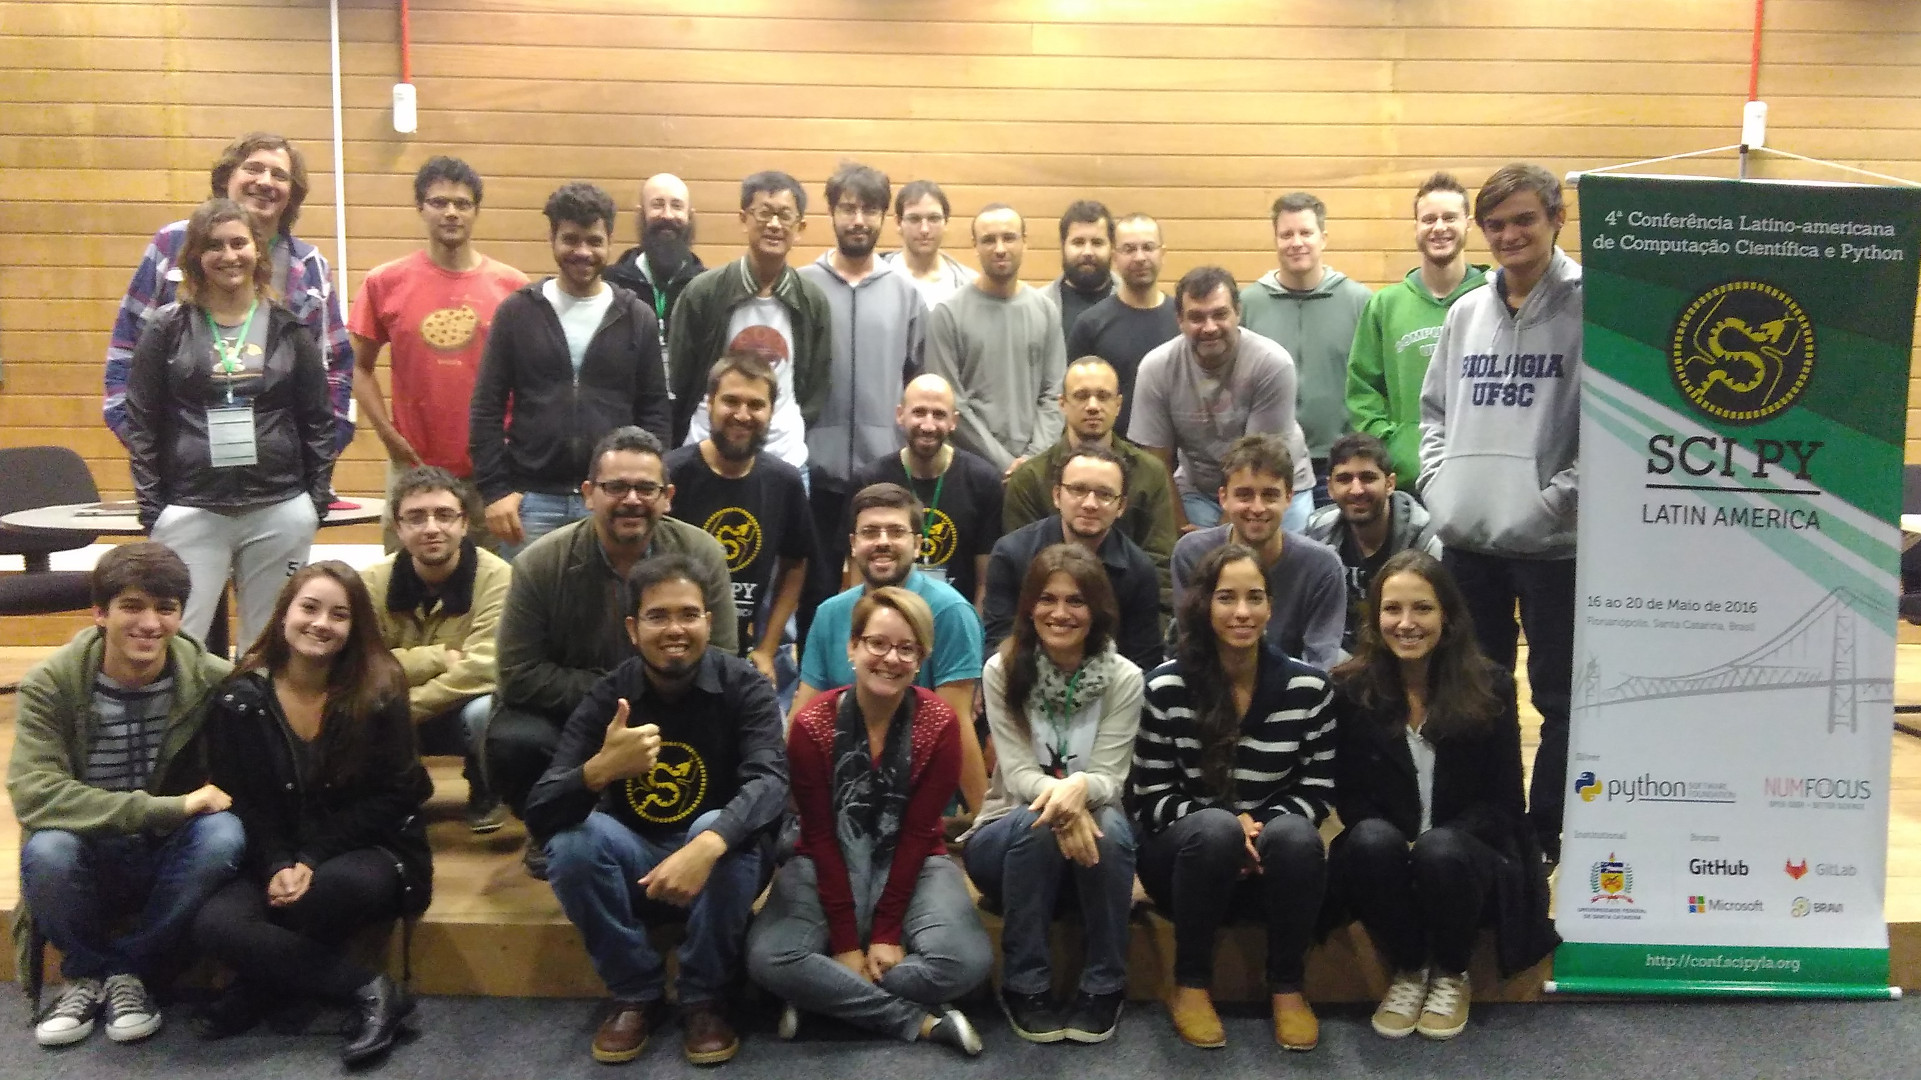
\includegraphics{group.jpg}

O SciPy Latin America 2016 recebeu mais de 160 inscritos paras as palestras e
uma média de 20 inscritos em cada um dos tutoriais que foram oferecidos.
Nas palestras tivemos um público médio de 50 pessoas. Nos tutoriais o público
variou bastante.

As inscrições nos tutoriais e palestras eram gratuitos. Embora a taxa de
ausentes seja alta ela está dentro de valores relatados por outros eventos
similares.

Para os próximos eventos estamos planejando cobrar inscrições com o objetivo de
aumentar a presença.

O número de mulheres no evento foi de 10\%. Uma taxa baixa mas que está na média
para eventos do tipo.

\newpage

\section*{Repercussão}

\newpage

\section*{Finanças}

\newpage

% Cover
\newgeometry{left=0cm, bottom=0cm, top=0cm, right=0cm}
\thispagestyle{empty}
\noindent  % To remove the unwanted white space.

\includegraphics{../../assets/contra-capa}
\NoBgThispage


\end{document}
